\vspace{-6px}
\section{Experiments}\label{sect:experiments}
\vspace{-4px}

The design of Learning@home was driven by two key assumptions: first, that MoE-based architectures can maintain high throughput under latency and second, that they can converge despite the presence of stale gradients. In this section we run several benchmarks in order to verify these assumptions. We intentionally focus on small-scale experiments to make them easier to reproduce and analyze. While solving practical vision and NLP problems is certainly our end goal, choosing a particular task would make it much harder to understand the general properties of our approach.

\vspace{-6px}
\subsection{Model throughput}\label{sect:exp_throughput}
\vspace{-4px}

Our first benchmark evaluates the performance of asynchronous training schemes under latency. We quantify this with training throughput, i.e., the number of training batches processed per second.
To emulate the distributed training environment, we create a model from a large number of identical blocks distributed evenly across 4 NVIDIA GTX 1080 GPUs. 
We simulate network latency by adding an artificial delay after computation of each block. The delay time is sampled from the exponential distribution, which was shown to model latency well \cite{sukhov2016generating}.%

\vspace{-1px}

Since our model size exceeds the memory limits of a single consumer GPU, the only mainstream paradigm that can compete with Learning@home is model parallel training. We also report the ``upper bound'' on training throughput by running the same computations with no network delays in a model parallel regime with pipelining similar to~\cite{huang2019gpipe}. For Learning@home, we use 64 trainer processes to send requests to the runtime processes\footnote{See the full setup: \url{https://github.com/mryab/learning-at-home\#running-the-experiments}}.

\vspace{-1px}

To measure the effect on blocks with different computation to communication ratio, we evaluate two popular block architectures. The first architecture is composed of $224$ feed-forward blocks, each having hidden dimensions of $1024\to4096\to4096\to 1024$ with layer normalization and ReLU activations in between. These blocks are treated as separate ``experts'' and process batches of size $2048$. The second architecture consists of $224$ BERT-like Transformer blocks \cite{bert} with hidden dimension 1024 and GELU activations \cite{hendrycks2016gaussian} applied to sequences of length $512$ with batch size $4$.

\vspace{-1px}

With this setup in mind, we can measure the throughput of the entire model as the time it takes to process 10 batches and dividing it by the total number of processed examples. These experiments were repeated 5 times for all methods to measure the mean and standard deviation of throughput.

\vspace{-1px}

Figure~\ref{fig:throughput} demonstrates that even with delay times approaching 200ms the asynchronous scheduler we have implemented as part of Learning@home maintains nearly the same throughput. In turn, model-parallel training throughput quickly degrades under latency, which is not surprising as it was not designed with slow communication in mind. %

\vspace{-1px}

To verify the validity of our conclusions, we have conducted similar experiments on cloud GPU instances in different regions.
This allows us to measure performance in a non-simulated scenario closer to the desired area of application.
In particular, we rented 3 instances with Tesla K80 hosted in West US, East US, and West Europe with average network latency of $92.49\pm32.42$ ms. The throughput values in Table \ref{tab:cloudk80} are similar to results for simulated latencies~(Figure \ref{fig:throughput}). 

\vspace{-1px}
Finally, we tested the scalability of our infrastructure by deploying DHT nodes in the same cloud regions and measuring the latency of beam search~(batch size 64, see Appendix C). Finding top-4 experts took $317\pm58$ms for 100 nodes, $528\pm127$ms for 1,000 nodes and $764\pm106$ms for 10,000 DHT nodes.

\begin{figure}[h]
\vspace{-2px}
    \hspace{-24px}\begin{minipage}{0.6\textwidth}
        \centering
        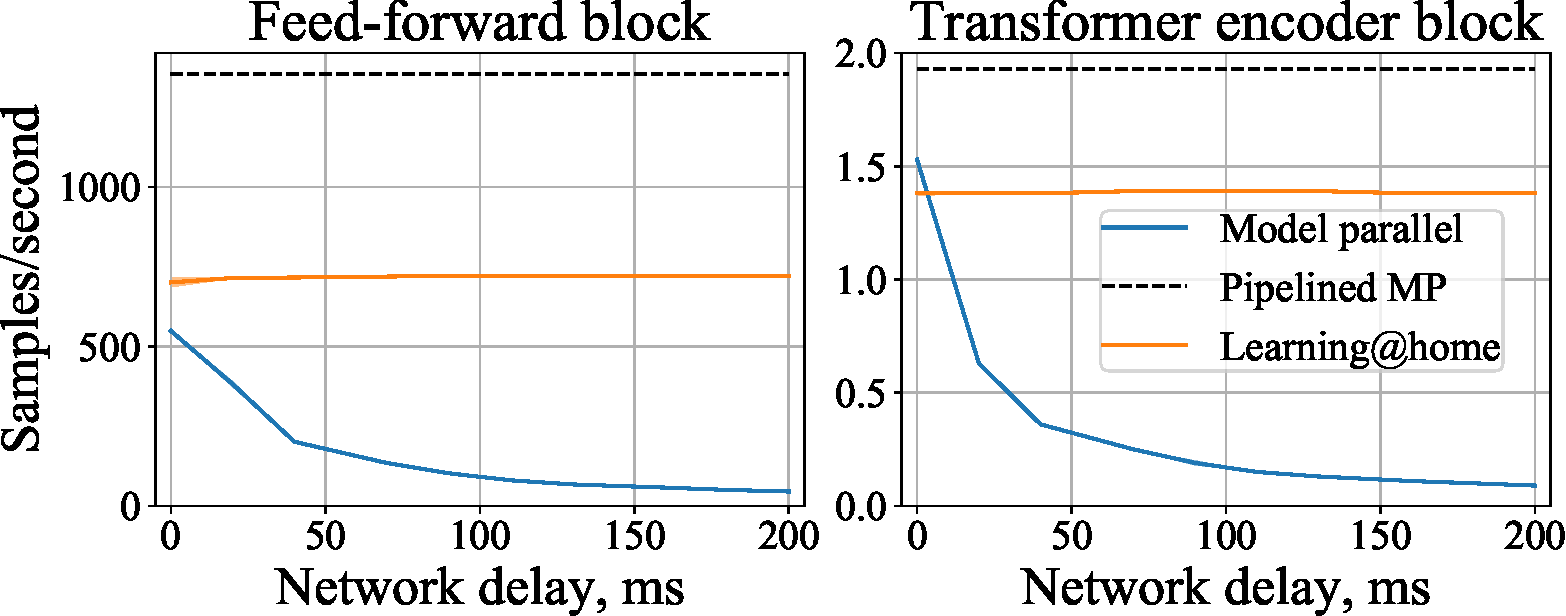
\includegraphics[width=210px]{resources/throughput_new.pdf}
        \captionof{figure}{Throughput with simulated latency.}
        \label{fig:throughput}
    \end{minipage}
    \hspace{-10px}
    \begin{minipage}{0.48\textwidth}
        \setlength{\tabcolsep}{2pt}
        \begin{tabular}{ccc}
        \toprule
        \multirow{2}{*}{Approach} & \multirow{2}{*}{Feed-forward}    & Transformer \\
                                  &            & encoder \\
        \midrule
        Model parallel & $7.23 \pm 0.06$ & $0.01 \pm 0.001$\\
        Learning@home  & $300.8\pm 15.9$  & $0.68 \pm 0.01$\\
        \bottomrule
        \end{tabular}
        \captionof{table}{Throughput (samples/s) for 3 cloud K80 in East US, West US and West Europe.}
        \label{tab:cloudk80}
    \end{minipage}
\end{figure}

\vspace{-16px}

\subsection{Convergence}\label{sect:exp_convergence}
\vspace{-4px}

Our second experiment aims to verify the robustness of DMoE to delayed updates.
For this goal, we choose one of the simpler tasks in deep learning, namely the MNIST digit recognition dataset \cite{mnist}, and compare convergence rates under varying network latency. All modern architectures can reliably solve this task, making it easier for us to isolate the effect of gradient staleness.

We evaluate four models: a traditional feed-forward model and three DMoE variations with different numbers of experts. The feed-forward network (FFN) consists of 4 stacked feed-forward blocks. Each block architecture is same as described in Section~\ref{sect:exp_throughput}, but with half as many hidden units. In turn, its DMoE counterparts have four DMoE layers, each composed of blocks with 1/4 of the FFN size. Both DMoE-based models use only 4 experts at a time regardless of their total number, hence being computationally equivalent to the FFN baseline.

We train all models asynchronously in high-latency and low-latency scenarios, using the same distribution for delay. In the high-latency scenario, each of 64 workers is delayed for 1 second on average while processing a batch. This corresponds to 125ms for each forward and backward pass through DMoE. For low latency emulation, we use 16 workers and 100ms average delay. The third experiment simulates node failure: each expert does not respond to a request with probability 0.1.

The results are presented in Figure \ref{fig:convergence_mnist}; as expected, the plots demonstrate that the higher latency scenario is more difficult for all models. However, the degree to which it affects the performance of DMoE architectures is much lower, especially for the largest of mixtures.

\begin{figure}[h]
\vspace{-6px}
    \begin{minipage}{0.99\textwidth}
        \hspace{-16px}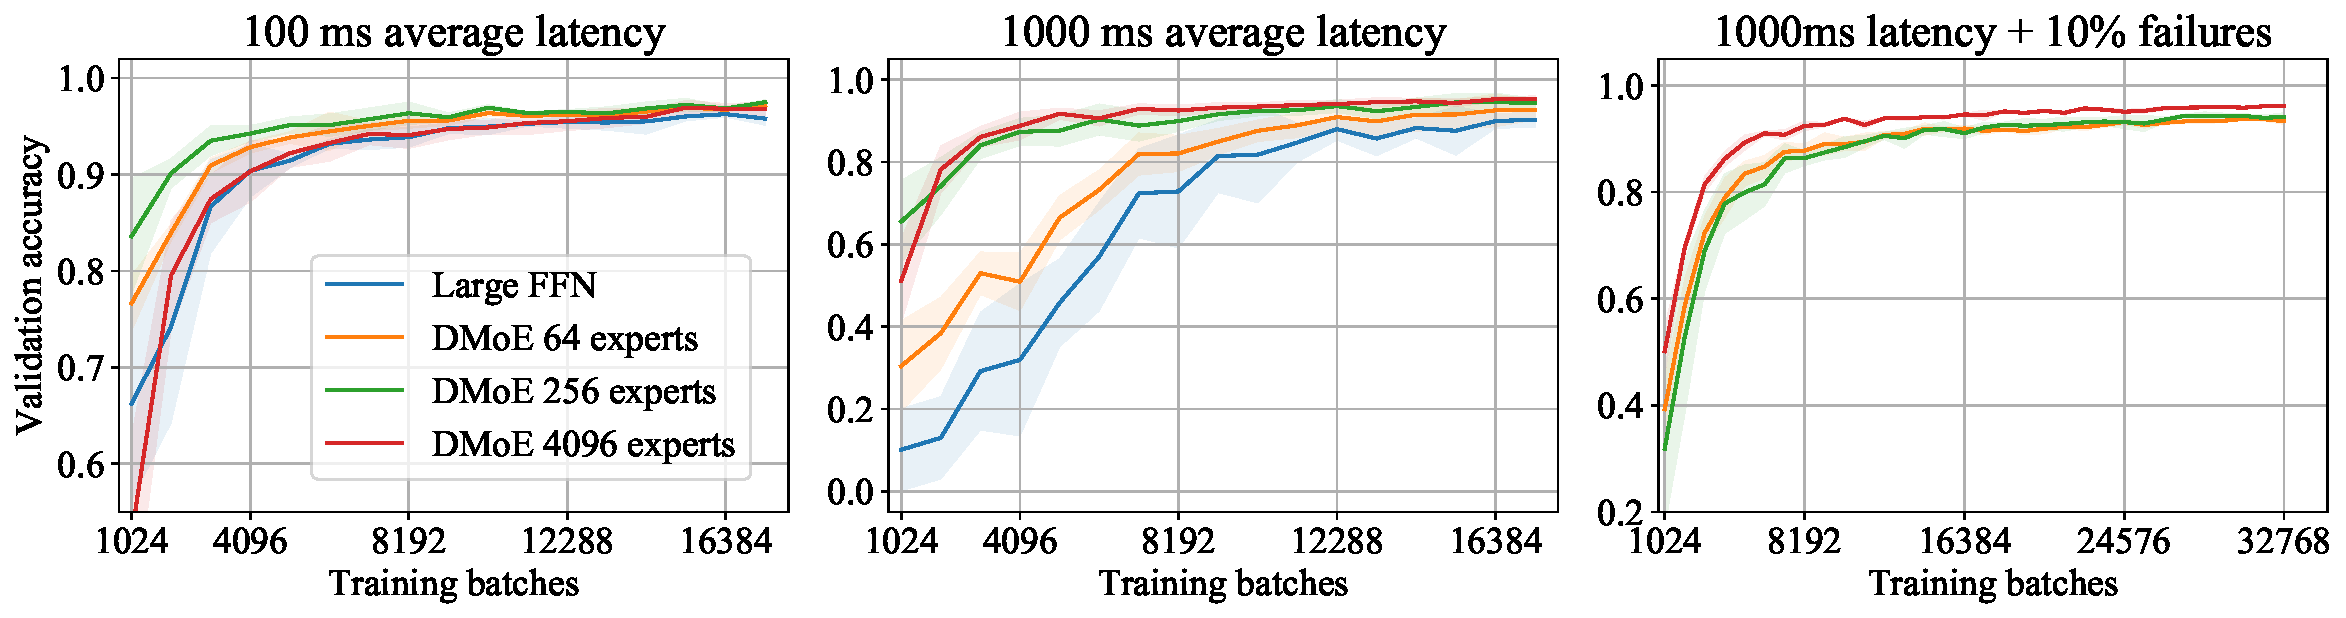
\includegraphics[width=417px]{resources/convergence.pdf}
    \end{minipage}
    \vspace{-4px}
    \captionof{figure}{Convergence plots for feedforward models with different network latencies and failure rates. Pale areas on depict unbiased standard deviations over 5 runs.}
    \label{fig:convergence_mnist}
\end{figure}

\vspace{-4px}

\subsection{Language models}\label{sect:exp_lm}

The third and final benchmark is neural language modeling. Specifically, we train Transformer-XL~\cite{dai2019transformer} on the WikiText-2~\cite{wikitext2} dataset. Both baseline and DMoE models use official recommended parameters with additional regularization proposed in \cite{dettmerswikitext2}.

The \texttt{base} model contains $16$ Transformer layers with the hidden size of $400$ and $900$ units in the feedforward layer. We also train a \texttt{small} baseline model with $200$ hidden and $450$ feedforward units. Our DMoE Transformer uses $256$ experts split evenly between $16$ layers. Each expert is a Transformer layer with the same dimensions as layers of the \texttt{small} baseline model. The DMoE layers route to top-$4$ experts, making our model roughly equivalent to \texttt{base} in terms of FLOPs per sample. Similarly to Section~\ref{sect:exp_convergence}, we train DMoE with 32 trainers (batch size 1 each), $1000$ms average latency, and $10\%$ failure rate.

\begin{figure}[h]
\vspace{-2px}
    \centering
        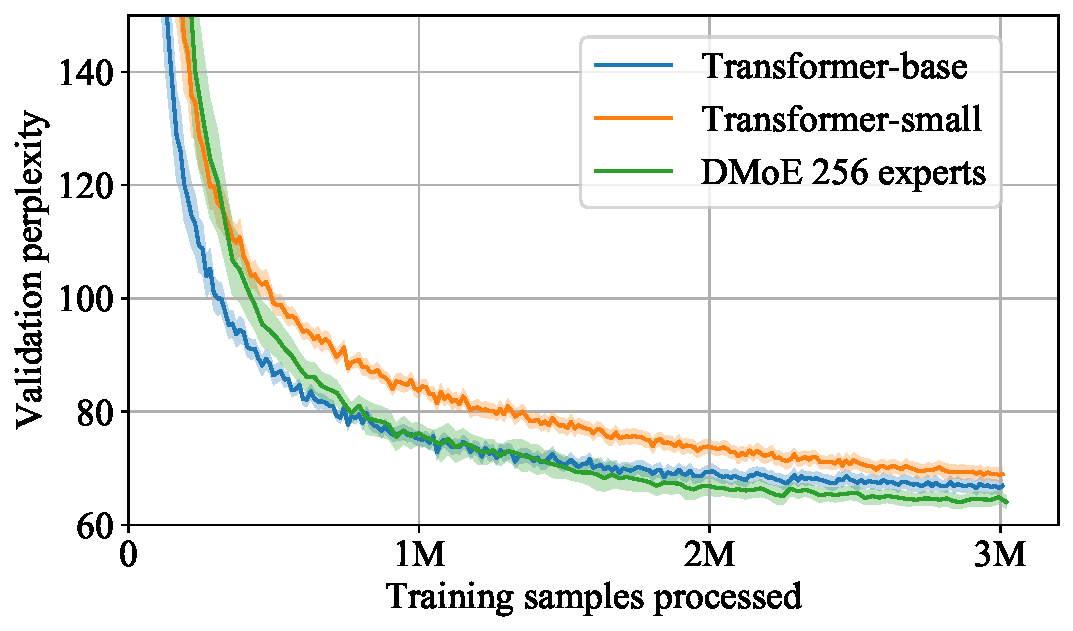
\includegraphics[width=0.5\textwidth]{resources/convergence_wikitext.pdf}
    \captionof{figure}{Convergence plots for Transformer language models on the WikiText-2 dataset. Pale areas on depict unbiased standard deviations over 5 runs.}
    \label{fig:convergence_lm}
\end{figure}

The results depicted in Figure~\ref{fig:convergence_lm} demonstrate a similar pattern to what was previously observed on feedforward networks. Curiously enough, we found that in this specific scenario the $10\%$ failure rate has a positive effect on the DMoE performance. We attribute this effect to a form of dropout regularization that prevents our model from overfitting the limited training data.
